% Beyond Query Linearity -- retuning the linear baseline at GPT-3 Large.
% NeurReps extended-abstract track (non-archival).
% JMLR/PMLR class. Working write-up for the collaboration (Marko et al.) --
% NOT anonymized: real names + run provenance so results can be merged/verified.
% Compile in this folder (needs jmlr.cls, jmlrutils.sty), plus booktabs.
% Figures live in figures/ (vector PDFs), built by code/make_figures.py from logs/.
% Every number quoted here is printed by code/analysis.py; nothing is hand-entered.
\documentclass[mlabstract,onecolumn]{jmlr}

\usepackage{booktabs}

\graphicspath{{figures/}}

\title[Retuning the Linear Baseline at GPT-3 Large]%
{Retuning the Linear Baseline at GPT-3 Large:\titlebreak
 What the Learning Rate Was Hiding}

% Working draft for the collaboration -- real names (Marko assembles the
% final author list / anonymizes before any review submission).
\author{\Name{Simon Sang}}

\begin{document}

\maketitle

\begin{abstract}
The reported advantage of the residual (nonlinear) query at GPT-3 Large was measured
against a linear baseline running at the GPT-3 default learning rate,
$2.5\times10^{-4}$, which is close to the highest rate the un-normalized linear model
survives. I stabilized that arm with QK-normalization and then swept its learning rate.
It reaches $2.5403$ at $1.5\times10^{-3}$, which is $0.076$ below the same arm at the
default rate and below all three of my residual-GELU runs ($2.5464$ to $2.5487$). So the
headline architecture gap does not survive giving the linear arm its own tuned rate, and
I read the earlier deltas as recipe-level rather than architectural. Two further results
qualify that. First, run-to-run spread is arm-dependent: two seeds of the stabilized
linear arm land $0.0002$ apart, while the residual arm spreads $0.0015$ over the same
change, so ``how many sigma'' depends entirely on which arm supplies the sigma. Second, a
residual variant that normalizes the query per head and drops the customary halving of
the attention scale reaches $2.5383$, the best number in the project, ahead of the tuned
linear arm by $0.0020$ at matched rate. That margin is $10\times$ the linear arm's seed
spread but only $1.3\times$ the residual arm's, so it is promising and not yet a win. I
also report what decay-to-zero costs in stability at this scale, where the plain arm
diverged at $1\times10^{-3}$ yet ran to completion at $2\times10^{-3}$. That completed run
reaches $2.5504$ with no normalization of any kind, closing $88\%$ of the distance between
the plain arm's own default-rate run and the swept optimum, which points at the optimization
recipe, schedule together with rate, rather than at the rate by itself.
\end{abstract}

\section{Setup}
\label{sec:setup}

\paragraph{Shared training protocol.} All runs use the same nanoGPT-based codebase on
OpenWebText (GPT-2 BPE, $9.036$B training tokens) with a fixed, precomputed
\emph{deterministic} batch-index ordering, tied input/output embeddings, context length
$1024$, and $60{,}002$ optimizer steps. Optimization is AdamW ($\beta_1=0.9$,
$\beta_2=0.95$), $2000$-step linear warmup, weight decay $0.1$, gradient clipping $1.0$,
precision bf16. Effective batch is $480$ sequences per step, so $491{,}520$ tokens per
step, within $2\%$ of the $0.5$M tokens GPT-3 Large itself used \citep{brown2020gpt3}.
GPT-3 Large is $24$ layers, $d_\text{model}=1536$, $16$ heads, $d_\text{head}=96$. The
model-initialization seed is fixed at $1337$; the batch-ordering seed is what varies, and
is named per run. Evaluation indices are precomputed per iteration, so at a given step
every run sees the \emph{identical} validation batch: same-step comparisons between runs
are therefore paired, which is what makes the small margins below readable at all.

\paragraph{Attention scale, and why it appears in the table.} The residual query is
$Q(X)=\tfrac{1}{2}(X+f_\theta(X))$ \citep{karbevski2026wkwv}. In the implementation the
code computes $q = X + \mathrm{LN}(f_\theta(X))$ with no explicit factor, and the
$\tfrac{1}{2}$ is folded into the attention scale, so the residual arm runs at
$\text{scale}=1/(2\sqrt{d_\text{head}})$ and the linear arm at $1/\sqrt{d_\text{head}}$.
I write this as a multiplier $s$ on the standard scale ($s=0.5$ and $s=1$). It is
recorded per run in Table~\ref{tab:runs} because one run departs from it, but it is
\emph{not} an uncontrolled difference between the arms: at $s=0.5$ the residual arm is
the method as defined.

\paragraph{Divergence guard.} Runs stop themselves. The training loop aborts on a
non-finite loss, or after two consecutive evaluations more than $0.5$ above that run's own
running-minimum validation loss. Every ``diverged'' entry below is that guard firing, not
a crash and not a manual kill, so the stopping step is comparable across runs.

\paragraph{Runs contributed here.} Table~\ref{tab:runs} lists every run in this note with
the settings read back from the loaded-config dictionary the trainer writes to each job's
log, rather than from the config filename. Figure~\ref{fig:curves} shows the learning-rate
sweep's train and validation curves.

\paragraph{Provenance.} Training code is the group repository,
\texttt{beyond\_query\_linearity}: the loop, learning-rate schedule and divergence guard in
\texttt{train.py}, and the query modes, attention scale and the QK- and k-normalization
options in \texttt{model.py}. Each run is one generated config under \texttt{configs/},
named for its arm and rate, submitted through \texttt{train\_seed.sbatch}. Configs are built
programmatically and re-imported before submission rather than hand-edited, so the file on
disk is the file that ran. The job identifiers in Table~\ref{tab:runs} index the cluster
logs, and the per-step losses those logs contain are the \texttt{logs/} directory
accompanying this note; every figure and every number quoted here is derived from them by
the two scripts in \texttt{code/}, so nothing in this write-up is transcribed by hand.

\begin{table}[ht]
\centering
\footnotesize
\setlength{\tabcolsep}{4pt}
\begin{tabular}{llccccclr}
\toprule
Job & Query & Norm. & $s$ & Peak LR & Min LR & Order & Sched. & Final val \\
\midrule
\multicolumn{9}{l}{\emph{GPT-3 Large}, linear query, the learning-rate sweep} \\
$8952$  & linear   & none    & $1$ & $2.5$e-$4$  & $2.5$e-$5$ & $42$ & cosine & $2.6247$ \\
$9645$  & linear   & QK-norm & $1$ & $2.5$e-$4$  & $2.5$e-$5$ & $43$ & cosine & $2.6165$ \\
$9776$  & linear   & QK-norm & $1$ & $7.5$e-$4$  & $1$e-$5$   & $43$ & cosine & $2.5551$ \\
$\mathbf{9777}$ & linear & QK-norm & $1$ & $\mathbf{1.5}$e-$\mathbf{3}$ & $1$e-$5$ & $43$ & cosine & $\mathbf{2.5403}$ \\
$9924$  & linear   & QK-norm & $1$ & $1.5$e-$3$  & $1$e-$5$   & $44$ & cosine & $2.5405$ \\
$9778$  & linear   & QK-norm & $1$ & $2.55$e-$3$ & $1$e-$5$   & $43$ & cosine & $2.5469$ \\
\midrule
\multicolumn{9}{l}{\emph{GPT-3 Large}, residual-GELU query} \\
$9436$  & res-GELU & none    & $0.5$ & $2.55$e-$3$ & $2$e-$5$ & $43$ & cosine & $2.5472$ \\
$9647$  & res-GELU & none    & $0.5$ & $2.55$e-$3$ & $2$e-$5$ & $44$ & cosine & $2.5487$ \\
$9780{+}10127$ & res-GELU & none & $0.5$ & $2.55$e-$3$ & $2$e-$5$ & $45$ & cosine & $2.5464$ \\
$\mathbf{9944}$ & res-GELU & \textbf{k-norm/ph} & $\mathbf{1}$ & $1.5$e-$3$ & $1$e-$5$ & $43$ & cosine & $\mathbf{2.5383}$ \\
\midrule
\multicolumn{9}{l}{\emph{GPT-3 Large}, plain linear under decay-to-zero} \\
$10140$ & linear   & none    & $1$ & $1$e-$3$    & $\mathbf{0}$ & $43$ & \textbf{D2Z} & div.\ $25$k \\
$\mathbf{10141}$ & linear & none & $1$ & $\mathbf{2}$e-$\mathbf{3}$ & $\mathbf{0}$ & $43$ & \textbf{D2Z} & $\mathbf{2.5504}$ \\
\midrule
\multicolumn{9}{l}{\emph{GPT-3 small}, decay-to-zero learning-rate sweep at $60$k} \\
$10130$ & linear   & none    & $1$ & $6$e-$4$    & $0$ & def. & D2Z & $2.9311$ \\
$10131$ & linear   & none    & $1$ & $1.2$e-$3$  & $0$ & def. & D2Z & $2.9053$ \\
$10132$ & linear   & none    & $1$ & $2.4$e-$3$  & $0$ & def. & D2Z & $2.8994$ \\
$\mathbf{10133}$ & linear & none & $1$ & $\mathbf{4.8}$e-$\mathbf{3}$ & $0$ & def. & D2Z & $\mathbf{2.8948}$ \\
$10134$ & linear   & none    & $1$ & $9.6$e-$3$  & $0$ & def. & D2Z & $2.9103$ \\
\midrule
\multicolumn{9}{l}{\emph{GPT-3 small}, the $180$k arm, first run under way} \\
$10135$ & linear   & none    & $1$ & $6$e-$4$    & $0$ & def. & D2Z & running \\
\bottomrule
\end{tabular}
\caption{Every run in this note. GPT-3 Large is $24$/$1536$/$16$ with
$d_\text{head}=96$; GPT-3 small is $12$/$768$/$12$, $d_\text{head}=64$,
$124.37$M parameters counted from the checkpoint with tied storage de-duplicated. $s$ is
the multiplier on the standard attention scale $1/\sqrt{d_\text{head}}$; $s=0.5$
implements the $\tfrac{1}{2}$ of the residual query (Section~\ref{sec:setup}). ``Order''
is the batch-ordering seed. Bold marks the two runs the argument turns on and the
settings that make them unusual. All settings were read from each job's logged config
dictionary. Per-step logs for every row are in \texttt{logs/}.}
\label{tab:runs}
\end{table}

\begin{figure}[ht]
\centering
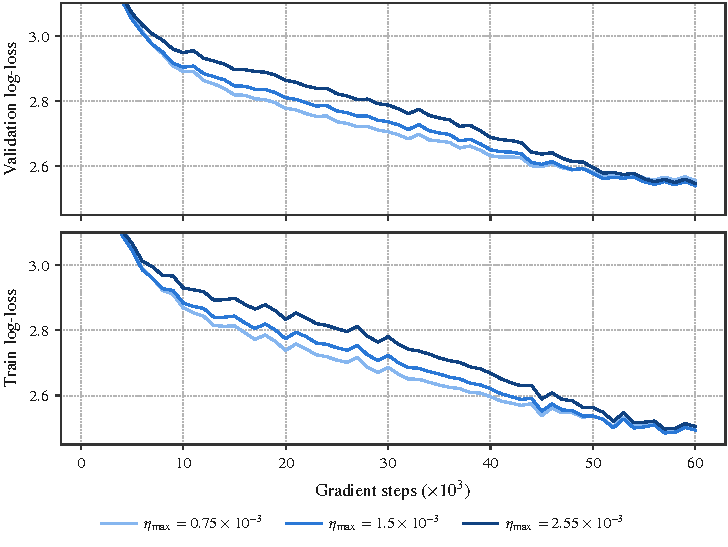
\includegraphics[width=\linewidth]{training_curves.pdf}
\caption{Validation and train log-loss for the three learning-rate sweep points on the
stabilized linear arm (step $0$ omitted for scale). Colour is a single ordered ramp, light
to dark, because peak learning rate is an ordered quantity rather than a set of categories.
The three curves are nearly indistinguishable until the final anneal, which is where the
sweep is decided.}
\label{fig:curves}
\end{figure}

\section{Sweeping the stabilized linear baseline}
\label{sec:sweep}

The linear baseline the architecture comparison used runs at the GPT-3 default
$2.5\times10^{-4}$ \citep{brown2020gpt3}. That is not a tuned setting for our recipe, it
is close to the ceiling of what the un-normalized linear model tolerates: at that rate the
plain arm completed on ordering seed $42$ but the guard stopped it on seeds $43$ and $44$.
QK-normalization \citep{dehghani2023vit22b,wortsman2023smallscale} removes that
instability, and once it is removed the rate can be swept. Figure~\ref{fig:ordering}, left,
shows both halves of that: three orderings of the plain arm at the default rate, two of
which the guard stopped, against the same arm and the same rate with QK-normalization
added, which completes. So the baseline was not merely untuned, it was at a setting where
tuning it was not yet possible.

Sweeping it moves the arm a long way (Figure~\ref{fig:bowl}). A quadratic in $\ln$ LR
through the three swept points puts the optimum at $1.56\times10^{-3}$ with curvature
$0.0276$ in loss per $(\ln \mathrm{LR})^2$, and the best measured point, $2.5403$ at
$1.5\times10^{-3}$, sits $0.076$ below the same arm at the default rate. For scale, that
$0.076$ is roughly $33$ times the entire spread of my three residual-GELU seeds.

The consequence for the architecture claim is direct. At its own tuned rate the linear arm
reaches $2.5403$, below all three residual-GELU runs ($2.5464$, $2.5472$, $2.5487$). At a
\emph{matched} rate of $2.55\times10^{-3}$ the two arms are indistinguishable: $2.5469$
for linear plus QK-norm against $2.5472$ for residual-GELU, a gap of $0.0003$. Neither
comparison leaves room for an architectural effect of the size originally reported. What
the residual query demonstrably does at this scale is tolerate, unmodified, a rate that
destroys the plain linear model; that is a real property, and it is a property of the
recipe rather than evidence of better features.

\begin{figure}[ht]
\centering
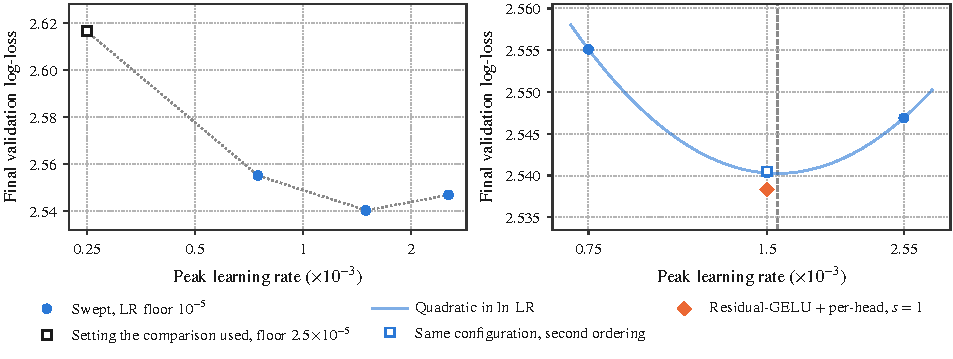
\includegraphics[width=\linewidth]{lr_sweep_bowl.pdf}
\caption{Final validation log-loss against peak learning rate for the stabilized linear
arm. Left, the full swept range: the open square is the setting the architecture comparison
used, $0.076$ above the swept optimum. Right, the same sweep zoomed, with the quadratic in
$\ln$ LR through the three swept points; the dashed vertical is its vertex at
$1.56\times10^{-3}$. The open square there is a second batch ordering at the same
configuration, $0.0002$ away, and the diamond is the per-head residual variant of
Section~\ref{sec:variant}, the only point below the fitted bowl. The run at
$2.5\times10^{-4}$ is excluded from the fit because it uses a different learning-rate
floor, $2.5\times10^{-5}$ against $1\times10^{-5}$.}
\label{fig:bowl}
\end{figure}

\section{Run-to-run spread is a property of the arm}
\label{sec:seed}

Every margin above is small enough that the noise floor decides whether it means anything,
and there is no single noise floor. Rerunning the stabilized linear arm at
$1.5\times10^{-3}$ under a different batch ordering gives $2.5405$ against $2.5403$, a
spread of $0.0002$, and the two curves stay within $0.0013$ of each other over the last
eleven evaluations. The residual arm under the same change of ordering gives $2.5472$
against $2.5487$, a spread of $0.0015$, and $0.0023$ across three orderings. The same
absolute gap is therefore worth $7.5$ times as many standard deviations on one arm as on
the other, so any claim of the form ``$n$ sigma'' has to name the arm it borrowed its
sigma from. Where I quote both below, that is why.
Figure~\ref{fig:ordering}, right, puts the two spreads on one axis.

\begin{figure}[ht]
\centering
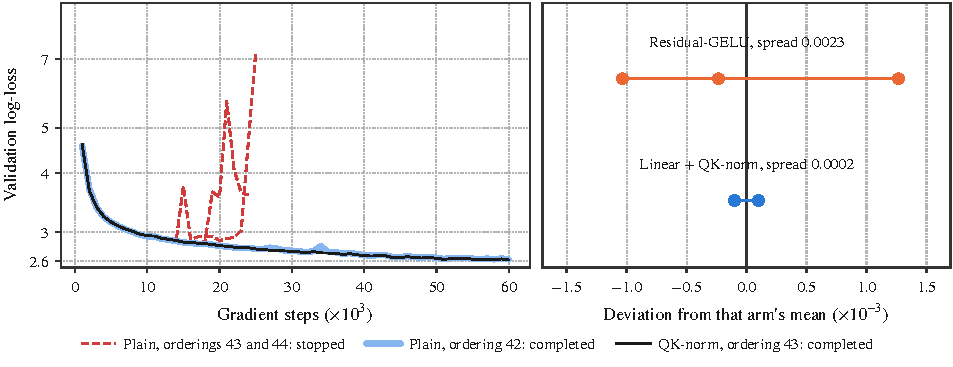
\includegraphics[width=\linewidth]{ordering_sensitivity.pdf}
\caption{Changing only the batch ordering. Left, at the GPT-3 default rate of
$2.5\times10^{-4}$ the plain linear arm completes on ordering seed $42$ and the guard stops
it on $43$ and $44$; QK-normalization at the same rate completes, and lands almost on top
of the one plain run that survived, which is drawn thick and pale underneath it so both are
visible. Right, once the instability is removed, how far apart
orderings land, per arm: $0.0002$ over two orderings for linear plus QK-norm against
$0.0023$ over three for residual-GELU. Each arm is centred on its own mean, because the gap
between the two means is $35$ times the smaller of the two spreads and an absolute axis
renders that spread invisible. The noise floor that decides every margin in this note is
itself arm-dependent.}
\label{fig:ordering}
\end{figure}

\section{A per-head residual variant, and where the arms differ}
\label{sec:variant}

One residual run departs from the method as defined. It normalizes the anchor and the
correction \emph{per head} rather than globally, which hard-bounds $|q_h|$ instead of
bounding it in expectation, and with that bound in place it drops the halving, running at
$s=1$. At the same rate, floor, ordering and schedule as the tuned linear arm, it reaches
$2.5383$: the best number in the project, and $0.0020$ ahead of $9777$.

By the previous section that $0.0020$ is $10\times$ the linear arm's seed spread and
$1.3\times$ the residual arm's. It is the most encouraging result here and it is not yet a
win; a seed replicate of this configuration is the single most valuable run outstanding.

Figure~\ref{fig:arm} shows where the difference lives. The residual arm is behind the
linear arm for $18$ of $60$ evaluations, trailing from step $2000$ to step $21000$, and
takes the lead only over the second half. A recipe that runs hot and then anneals produces
exactly this shape, which is a further reason to read these margins as optimization
effects until a replicate says otherwise.

The train side rules out one reading of that win. It is not better generalization: the
variant leads on \emph{train} loss by $0.0028$, slightly more than its $0.0020$ validation
lead, and its train-to-validation gap is marginally the wider of the two, $0.0471$ against
$0.0463$. Whatever the per-head bound is buying, it is fitting the data a little better
rather than overfitting it a little less.

\begin{figure}[ht]
\centering
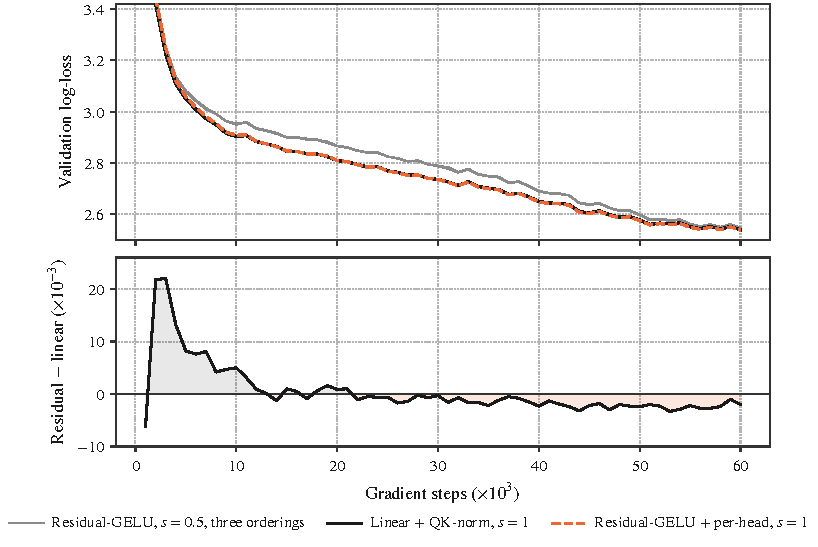
\includegraphics[width=\linewidth]{arm_matched.pdf}
\caption{The two arms at matched rate, floor, ordering and schedule, with my three
$s=0.5$ residual runs in grey for context. Above, validation log-loss over the whole run,
where the final $0.0020$ separation is far too small to read. Below, the difference between
them, which is what the panel is for: the residual arm trails by as much as $0.022$ through
the first fifth of training, crosses over around step $21$k, and leads by $0.0020$ at the
end. Shading marks which arm is ahead.}
\label{fig:arm}
\end{figure}

\section{Does the optimal rate fall with the token budget?}
\label{sec:horizon}
\label{sec:tpp}

If the optimum moves with training length, then every comparison in this project inherits
a dependence on how long we train, and the $60$k-step numbers do not transfer. The
literature says the effect is real, but that tokens-per-parameter is the wrong variable
for it.

\citet{bjorck2024horizons} fit $\mathrm{LR}^*(N,D) = C N^{-0.23} D^{-0.32}$ and recommend
transferring a tuned rate across horizons by $D^{-0.32}$. That exponent is their pooled
fit for models of $760$M and up, and they restrict it to that regime because smaller
models show a steeper one; their per-model table gives $0.6531$ for their $125$m model,
which is exactly our GPT-3 small geometry. Better still, they publish the measured optima
for that model at six horizons, so the slope can be taken locally rather than from a
global fit. Our budgets, $29.5$B and $88.5$B tokens, both fall inside their $25$ to $100$B
segment, where the local slope is $0.51$ (Figure~\ref{fig:horizon}). Tripling the budget
should therefore move the optimum down by about $1.75\times$, which at the curvature
measured in Section~\ref{sec:sweep} costs $0.0087$ if the rate is not moved, roughly
$43\times$ the linear arm's seed spread.

Two qualifications matter. Their warmup is $\max(1000, 0.01\times\text{iters})$, so it
scales with the horizon, and \citet{filatov2024time} find that scaling warmup with the
horizon drifts the optimum on its own; our warmup is fixed at $2000$ steps, so part of
their exponent should not reproduce for us. And the variable is not tokens-per-parameter.
\citet{bergsma2025d2z} hold the step count fixed and raise the budget by growing the batch
instead, and the optimal rate then \emph{increases}; \citet{li2025steplaw} fit a positive
data exponent, $\eta \propto N^{-0.713} D^{+0.307}$, with batch co-scaled;
\citet{filatov2024time} attribute the sign to where the batch sits relative to a critical
batch size that itself grows with the horizon. Adding tokens by taking more steps at fixed
batch lowers the optimum; adding them by enlarging the batch raises it. Only the first is
our situation.

Two widely cited results are often read as supporting the tokens-per-parameter version and
do not. \citet{deepseek2024} fit the optimal rate against total compute and find it
falling as $C^{-0.125}$, but along their own compute-optimal frontier the parameter and
token exponents are $0.5243$ and $0.4757$, so tokens-per-parameter varies only as
$C^{-0.049}$: over the range on which they actually fit the rate it drops by $1.94\times$
while tokens-per-parameter barely moves, which records a size effect rather than a budget
one. Nor does the GPT-3 table support the reading: every
variant there saw $300$B tokens, so tokens-per-parameter is exactly inverse to parameter
count and the two cannot be separated \citep{brown2020gpt3}.

\begin{figure}[ht]
\centering
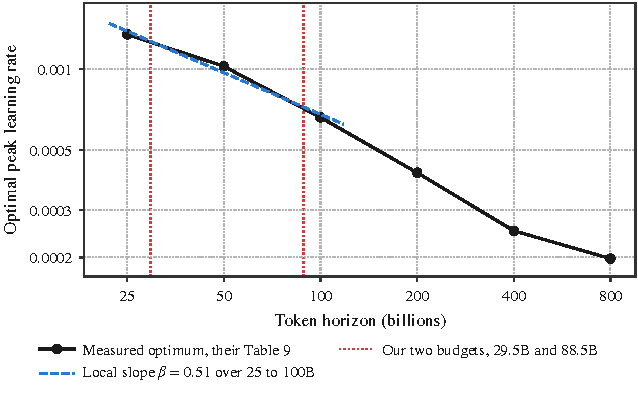
\includegraphics[width=0.62\linewidth]{lr_vs_horizon.pdf}
\caption{Measured optimal peak learning rate against token horizon for the $125$m model of
\citet{bjorck2024horizons}, which matches our GPT-3 small geometry. The slope steepens
with horizon, so the local slope over the segment containing our two budgets, $0.51$, is
the relevant one rather than their global fit.}
\label{fig:horizon}
\end{figure}

\section{Decay-to-zero at GPT-3 Large}
\label{sec:d2z}

\citet{bergsma2025d2z} argue for decaying the rate linearly to zero, and report that the
optimal peak is much more stable under that schedule than under decay to a tenth of peak,
shifting ``substantially lower for Constant, somewhat lower for $10\times$, and hardly at
all for D2Z''. Their own peak sits a factor of two \emph{above} the $10\times$ optimum at
matched budget. If that holds here it is convenient, because it means our tuned rate
transfers across budgets.

What it costs at this scale is stability, and the cost is not ordered in the rate
(Figure~\ref{fig:d2z}). Two runs of the plain linear arm under decay-to-zero, identical
except in peak rate and sharing an initialization and a data ordering: at
$1\times10^{-3}$ the run reached $2.8393$ at step $20$k, survived one spike at $18$k, and
then ran away, with the guard stopping it at $25$k; at $2\times10^{-3}$, twice the rate, the
run went the distance and finished at $2.5504$. The survivor also carried the \emph{larger}
attention logits, peaking at $486$ at layer $12$ against $274$ for the run that died, and
both stayed orders of magnitude below the $10^4$ threshold of
\citet{wortsman2023smallscale}. So on this arm divergence under decay-to-zero is not
monotone in the peak rate, and the logit norm does not predict which run survives.

That surviving run is the most consequential number in this note, because of what it does
\emph{not} have. It carries no QK-normalization, no $z$-loss, no per-head bound, nothing:
it is the same plain architecture that the guard stopped on two of three orderings at
$2.5\times10^{-4}$ under cosine. Changing only the schedule and the rate takes it from
$2.6247$ to $2.5504$. Measured from that same plain baseline, stabilizing the arm and then
sweeping its rate recovered $0.0844$; schedule and rate alone recover $0.0743$, which is
$88\%$ of it, and land below the $7.5\times10^{-4}$ point of that sweep ($2.5551$), within
$0.010$ of its optimum. The lesson I take is that Section~\ref{sec:sweep}'s
conclusion should be stated one notch wider than I first put it: what the original
comparison was missing is a tuned \emph{recipe}, schedule and rate together, and not merely
a tuned rate. It does not rescue the claim that decay-to-zero stabilizes this arm, since the
run at half the rate still died.

I note one thing about attributing such failures to precision. \citet{bergsma2025d2z}
report needing float32 to reach their higher optimum, but their appendix and their figure
caption disagree about whether the $16$-bit runs were bfloat16 or float16, and the strings
bf16, fp16 and fp32 appear nowhere in the paper, so the only precision it pins down
unambiguously is float32. Our failures are bf16 throughout; two of the plain-arm
divergences already carried a $z$-loss term and died anyway, while QK-normalization lifted
the usable rate on the same arm by more than tenfold in the same precision. That points at
logit growth rather than at mantissa bits.

\begin{figure}[ht]
\centering
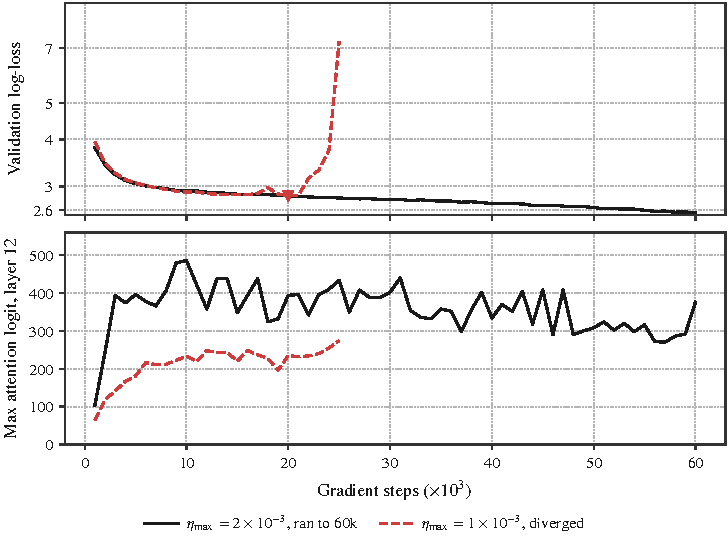
\includegraphics[width=\linewidth]{d2z_stability.pdf}
\caption{The two decay-to-zero runs on the plain linear arm, identical but for the peak
rate and sharing an initialization and a batch ordering. Above, validation log-loss: the
\emph{lower} peak rate is the one that diverged, reaching its minimum of $2.8393$ at step
$20$k (triangle) before running away, with the guard stopping it at $25$k, while the run at
twice that rate went the full $60$k and finished at $2.5504$ with no normalization of any
kind. Below, the maximum attention logit at layer $12$ for the same two runs; the survivor
carries the larger logits throughout, peaking at $486$ against $274$, and both stay three
orders of magnitude below the $10^4$ threshold of \citet{wortsman2023smallscale}.}
\label{fig:d2z}
\end{figure}

\section{The GPT-3 small sweep}
\label{sec:small}

To measure the horizon dependence in our own setup rather than borrowing an exponent, I am
sweeping five rates at two budgets on GPT-3 small under decay-to-zero, with everything
else matched: $60{,}002$ steps ($29.5$B tokens, $237$ tokens per parameter, $3.3$ epochs of
OpenWebText) and $180{,}000$ steps ($88.5$B tokens, $711$ per parameter, $9.8$ epochs). The
grid is $6\times10^{-4}$ to $9.6\times10^{-3}$ in factors of two, centred at
$2.4\times10^{-3}$ on two independent estimates: our GPT-3 Large optimum transferred down,
and the $125$m optimum of \citet{bjorck2024horizons} scaled up by the factor of two that
\citet{bergsma2025d2z} report between decay-to-zero and decay-to-a-tenth.

All five $60$k runs have now finished, and the sweep is bracketed
(Figure~\ref{fig:small}): $2.9311$ at $6\times10^{-4}$, $2.9053$ at $1.2\times10^{-3}$,
$2.8994$ at $2.4\times10^{-3}$, $2.8948$ at $4.8\times10^{-3}$, then back up to $2.9103$ at
$9.6\times10^{-3}$. A quadratic through the three points around the minimum puts the optimum
at $3.98\times10^{-3}$, with curvature $0.0209$ in loss per $(\ln \mathrm{LR})^2$, so this
bowl is about a quarter shallower than the GPT-3 Large one of Section~\ref{sec:sweep}.

The grid centre was therefore low by roughly a factor of two, and that is the useful
negative result, because \emph{both} estimates that produced it were low by that factor:
transferring our own GPT-3 Large optimum down, and scaling the $125$m optimum of
\citet{bjorck2024horizons} up by the factor of two that \citet{bergsma2025d2z} report
between decay-to-zero and decay-to-a-tenth. Two independent routes agreeing was not evidence
that either was right, and I had read their agreement as reassurance when I set the grid.

One methodological note, because reading this sweep early would have inverted the answer.
Under decay-to-zero the comparison is only meaningful between finished runs. At step $36$k
the ordering was \emph{exactly reversed}, monotone in the opposite direction: $3.0348$ at
$6\times10^{-4}$ rising steadily to $3.1948$ at $9.6\times10^{-3}$. The run that led at $36$k
finished last, and $4.8\times10^{-3}$, which finished first, was still fourth of five at
$54$k. The anneal reorders the whole field, and most of that happens in the last $6$k steps.
Any statement I make about which rate is best is a statement about completed runs only.

One caveat on interpreting these budgets against the literature. Our corpus is $9.036$B
tokens, so $60$k steps is already $3.3$ epochs and $180$k is $9.8$. Every study cited here
trains on effectively unique tokens; \citet{bjorck2024horizons} do test repetition, and
find that the horizon rather than the count of unique tokens sets the scaling, but their
test is a single appendix figure on a $50$m model reaching four epochs, which is the most
tested anywhere in that paper. Our $180$k point sits well past it, so I will report epochs
alongside tokens-per-parameter rather than treat the two as interchangeable.

The $180$k arm has started, with $6\times10^{-4}$ under way and past step $60$k, and having
the $60$k bowl bracketed makes that arm a sharp test rather than a second exploration.
Tripling the budget at the local slope of $0.51$ from Section~\ref{sec:horizon} should move
the optimum down by $1.75\times$, from $3.98\times10^{-3}$ to about $2.3\times10^{-3}$. The
grid centre I chose, $2.4\times10^{-3}$, happens to sit almost exactly there. So the same
centre that was low by a factor of two at $60$k is well placed at $180$k if the exponent
holds, and the prediction is falsifiable in the direction that matters: if the $180$k bowl
also minimizes near $4\times10^{-3}$, there is no horizon dependence to speak of under
decay-to-zero, which is what \citet{bergsma2025d2z} report and what the literature review
behind this note led with.

\begin{figure}[ht]
\centering
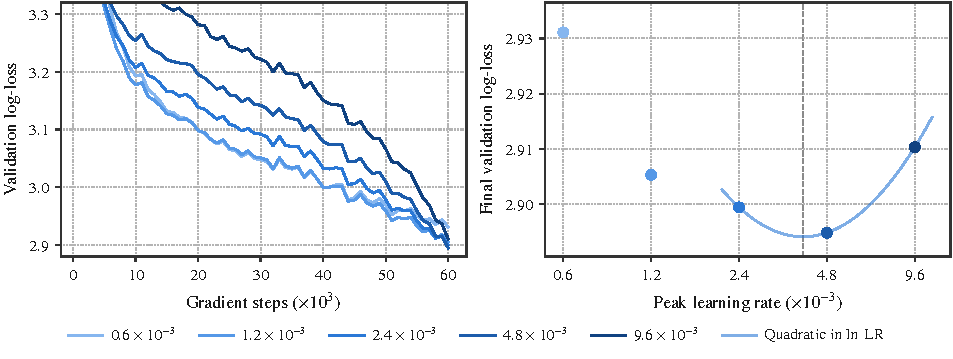
\includegraphics[width=\linewidth]{small_sweep_60k.pdf}
\caption{The $60$k-step GPT-3 small sweep under decay-to-zero, all five rates finished.
Left, validation log-loss per rate. Right, final loss against peak rate, with a quadratic in
$\ln$ LR through the three points around the minimum; the dashed vertical is its vertex at
$3.98\times10^{-3}$. The bowl is bracketed, and the grid centre of $2.4\times10^{-3}$ sits
about a factor of two below the optimum.}
\label{fig:small}
\end{figure}

\section{What I claim, and what I do not}

I claim that the optimization recipe, not the query mechanism, accounts for the reported gap
at GPT-3 Large. Stabilizing the linear arm and sweeping its rate takes it to $2.5403$, past
all three of my residual runs, and at a matched rate the two arms differ by $0.0003$.
Stronger, the plain arm with nothing added at all reaches $2.5504$ on a decay-to-zero
schedule at $2\times10^{-3}$, recovering $88\%$ of the gap without touching the architecture
or stabilizing anything. I claim that run-to-run spread differs by $7.5\times$
between the arms, so significance claims must name their arm. I claim that under
decay-to-zero on this arm, divergence is not monotone in the peak rate, and that the
attention-logit norm does not predict it.

I do not claim the nonlinear query is worthless. It tolerates an optimization regime that
destroys the plain linear model, which is what the earlier robustness results really
established, and the per-head variant of Section~\ref{sec:variant} is currently the best
configuration I have at $2.5383$. I do not claim that variant is a win: at $1.3\times$ the
residual arm's own seed spread it needs a replicate, which is the next run I would spend a
card on. I do not claim a horizon exponent for our setup. One of the two budgets is measured
and the other has a single run in it, and Section~\ref{sec:small} shows that reading this
sweep before the anneal finishes inverts the ordering, so the exponent waits for the second
budget.

\begin{thebibliography}{9}

\bibitem[Karbevski \& Mijoski(2026)]{karbevski2026wkwv}
Karbevski, M. and Mijoski, A.
\newblock {WK}, {WV} is ({L}inearly) All You Need: On the Necessity of the
  {QKV} Weight Triplet in Self-Attention Transformers.
\newblock In \emph{Workshop on Weight-Space Symmetries, 43rd International
  Conference on Machine Learning (ICML)}, Seoul, South Korea, 2026.
\newblock Extended versions: arXiv:2510.23912, arXiv:2603.13381, arXiv:2604.23705.

\bibitem[Brown et al.(2020)]{brown2020gpt3}
Brown, T., et al.
\newblock Language Models are Few-Shot Learners.
\newblock In \emph{NeurIPS}, 2020. arXiv:2005.14165.

\bibitem[Bjorck et al.(2024)]{bjorck2024horizons}
Bjorck, J., Benhaim, A., Chaudhary, V., Wei, F., and Song, X.
\newblock Scaling Optimal {LR} Across Token Horizons.
\newblock \emph{ICLR}, 2025. arXiv:2409.19913.

\bibitem[Bergsma et al.(2025)]{bergsma2025d2z}
Bergsma, S., et al.
\newblock Straight to Zero: Why Linearly Decaying the Learning Rate to Zero
  Works Best for {LLM}s.
\newblock arXiv:2502.15938, 2025.

\bibitem[Filatov et al.(2024)]{filatov2024time}
Filatov, O., Ebert, J., Wang, J., and Kesselheim, S.
\newblock Time Transfer: On Optimal Learning Rate and Batch Size in the
  Infinite Data Limit.
\newblock arXiv:2410.05838, 2024.

\bibitem[Li et al.(2025)]{li2025steplaw}
Li, H., et al.
\newblock Predictable Scale: Part {I}, Optimal Hyperparameter Scaling Law in
  Large Language Model Pretraining.
\newblock arXiv:2503.04715, 2025.

\bibitem[DeepSeek-AI(2024)]{deepseek2024}
DeepSeek-AI.
\newblock {DeepSeek} {LLM}: Scaling Open-Source Language Models with Longtermism.
\newblock arXiv:2401.02954, 2024.

\bibitem[Dehghani et al.(2023)]{dehghani2023vit22b}
Dehghani, M., et al.
\newblock Scaling Vision Transformers to 22 Billion Parameters.
\newblock In \emph{ICML}, 2023. arXiv:2302.05442.

\bibitem[Wortsman et al.(2023)]{wortsman2023smallscale}
Wortsman, M., et al.
\newblock Small-scale proxies for large-scale Transformer training instabilities.
\newblock arXiv:2309.14322, 2023.

\end{thebibliography}

\end{document}
